\subsection*{a)}
Die Matrix beschreibt den Messprozess, das ein Ereigniss nicht immer genau dem ``wahren'' bin zugeordnet werden kann. Es wird jeweils mit der Wahrscheinlichkeit $\nu$ einder den beiden daneben liegenden Bins zugeordnet. Dabei sind beide gleichwahrscheinlich.
\subsection*{b)}
Der übersichthalber werden hier nicht die Werte aufgetragen sondern. Die simmulierten gemessenen Ereignisszahlen gegen die wahre Verteilung in einem Histogramm zusammen aufgetragen. Die werte können der Python Datei entnommen werden falls sie erwünscht sind. 
\begin{figure}[H]
  \centering
  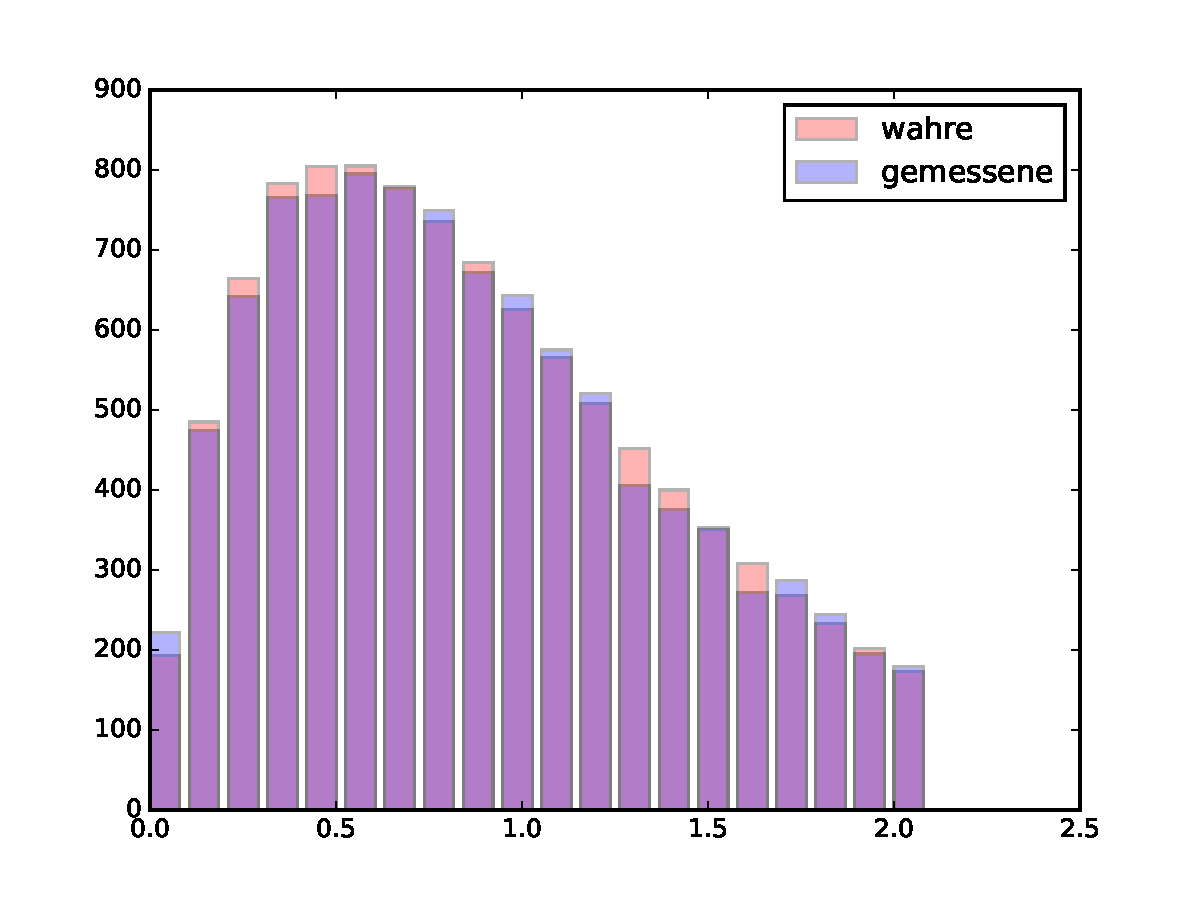
\includegraphics[width=\textwidth]{./Python/gemesseneVerteilung.pdf}
  \caption{wahre Ereignisszahlen und gemessene Ereignisszahlen}
\end{figure}
\subsection*{c)}
Kleine Eigenwerte können durch das Sotieren später einfacher Weggeworfen werden um Oszillationen zu vermeiden. Die Faltungsgleichung hatt nun die Gestalt 
\begin{equation}
  g = U \cdot D \cdot U^{-1} \cdot f
\end{equation}
\subsection*{d)}
Für große b Werte werden die Oszillationen bei der Faltung größer. Somit sind $b_i$'s unterhalb von 1 wünschenswert damit die Faltung nicht all zu stark oszilliert. 
\begin{figure}[H]
  \centering
  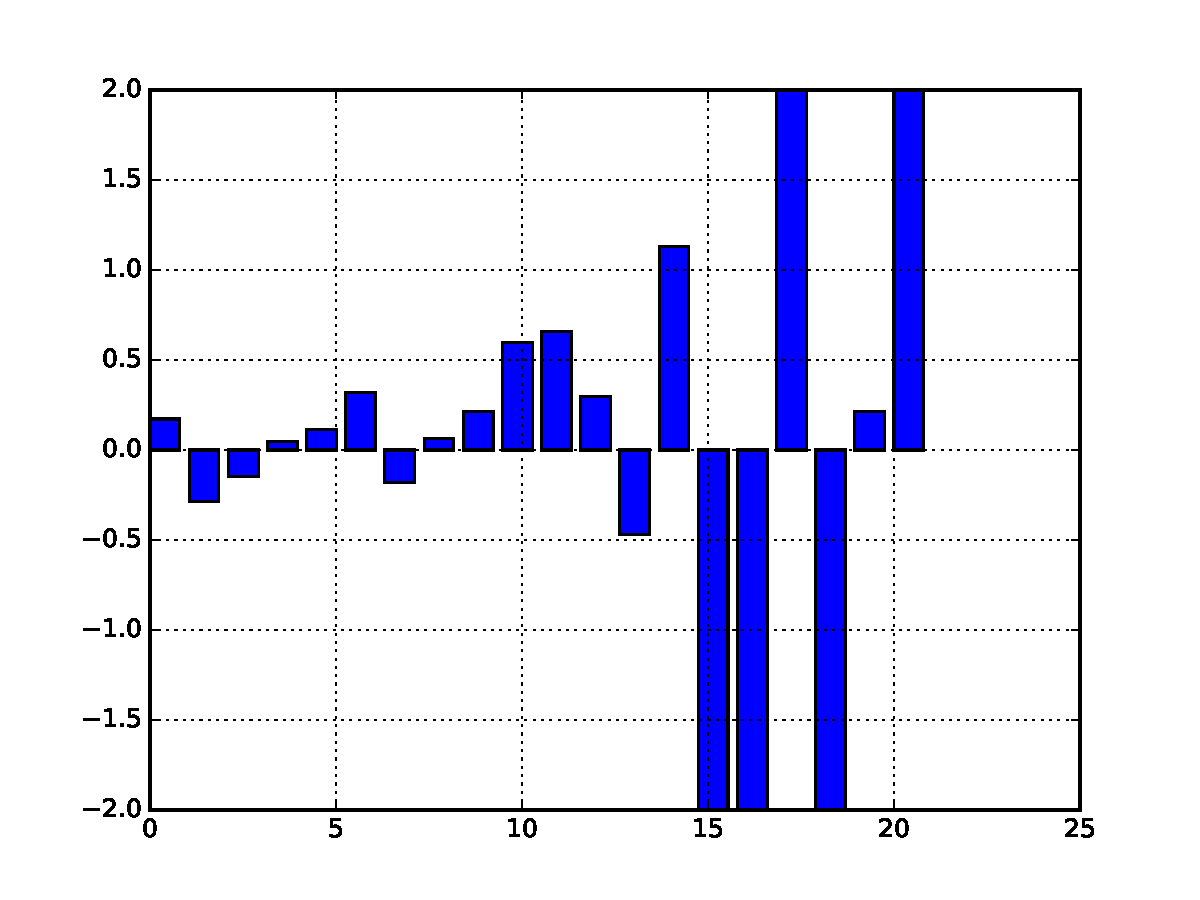
\includegraphics[width=\textwidth]{./Python/bar.pdf}
  \caption{Koeffizienten $b_i$}
\end{figure}
Die Matritzen und Vektoren sind aus dimensionsgründen wieder der Pythondatei zu entnehmen.
